\documentclass[tikz,border=2pt]{standalone}
\usepackage{amsmath,amssymb}
\usepackage{tikz}
\usepackage{pgfplots}
\pgfplotsset{compat=1.18}

\begin{document}
% Marginal expected cost G'(y) = (b+h)F(y) - b for uniform demand on [80,120], b = 3.3,
% h = 2.2: negative (stocking more helps) until F(y) = beta = 0.6 at y* = 104, positive after.
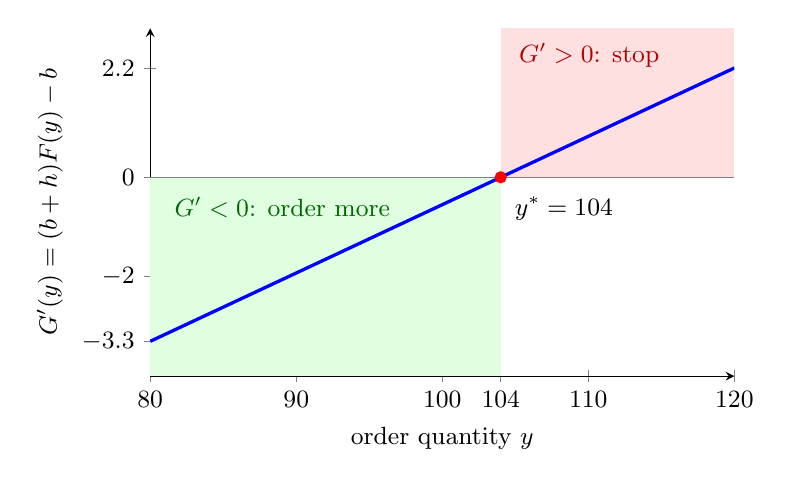
\begin{tikzpicture}
	\begin{axis}[width=9cm, height=6cm, xlabel={order quantity $y$}, ylabel={$G'(y)=(b+h)F(y)-b$}, xmin=80, xmax=120, ymin=-4, ymax=3, axis lines=left, tick label style={font=\small}, label style={font=\small}, xtick={80,90,100,104,110,120}, ytick={-3.3,-2,0,2.2}]
		\fill[green!12] (axis cs:80,-4) rectangle (axis cs:104,0);
		\fill[red!12] (axis cs:104,0) rectangle (axis cs:120,3);
		\draw[gray] (axis cs:80,0) -- (axis cs:120,0);
		\addplot[blue, very thick, domain=80:120] {5.5*(x-80)/40-3.3};
		\addplot[only marks, mark=*, mark size=2pt, red] coordinates {(104,0)};
		\node[anchor=north west, font=\small, green!40!black] at (axis cs:81,-0.2) {$G'<0$: order more};
		\node[anchor=north west, font=\small, red!70!black] at (axis cs:104.6,2.9) {$G'>0$: stop};
		\node[anchor=north west, font=\small] at (axis cs:104.3,-0.2) {$y^*=104$};
	\end{axis}
	\end{tikzpicture}
\end{document}
